\documentclass[tikz, border=10pt]{standalone}
\usepackage{tikz}
\usetikzlibrary{calc}

\begin{document}
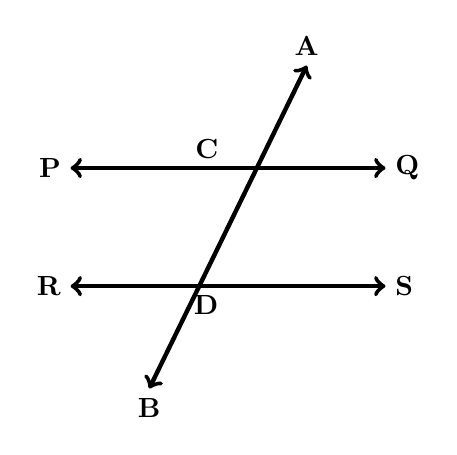
\begin{tikzpicture}

% Define points for upper parallel line PQ
\coordinate (P) at (0, 1.5);
\coordinate (Q) at (4, 1.5);
\coordinate (C) at (2, 1.5);

% Define points for lower parallel line RS
\coordinate (R) at (0, 0);
\coordinate (S) at (4, 0);
\coordinate (D) at (2, 0);

% Define points for transversal AB
\coordinate (A) at (3, 2.8);
\coordinate (B) at (1, -1.3);

% Draw upper parallel line PQ
\draw[ultra thick][<->] (P) -- (Q);

% Draw lower parallel line RS
\draw[ultra thick][<->] (R) -- (S);

% Draw transversal AB (through C and D)
\draw[ultra thick][<->] (A) -- (B);

% Labels
\node[above] at (A) {\textbf{A}};
\node[below] at (B) {\textbf{B}};
\node[left] at (P) {\textbf{P}};
\node[right] at (Q) {\textbf{Q}};
\node[left] at (R) {\textbf{R}};
\node[right] at (S) {\textbf{S}};
\node[above left] at (C) {\textbf{C}};
\node[below left] at (D) {\textbf{D}};

\end{tikzpicture}
\end{document}